% -*- coding: utf-8; -*-

\chapter{Código fonte do sistema}
\section{Tela Inicial do Sistema}
\begin{figure}[!h]
	\centering
	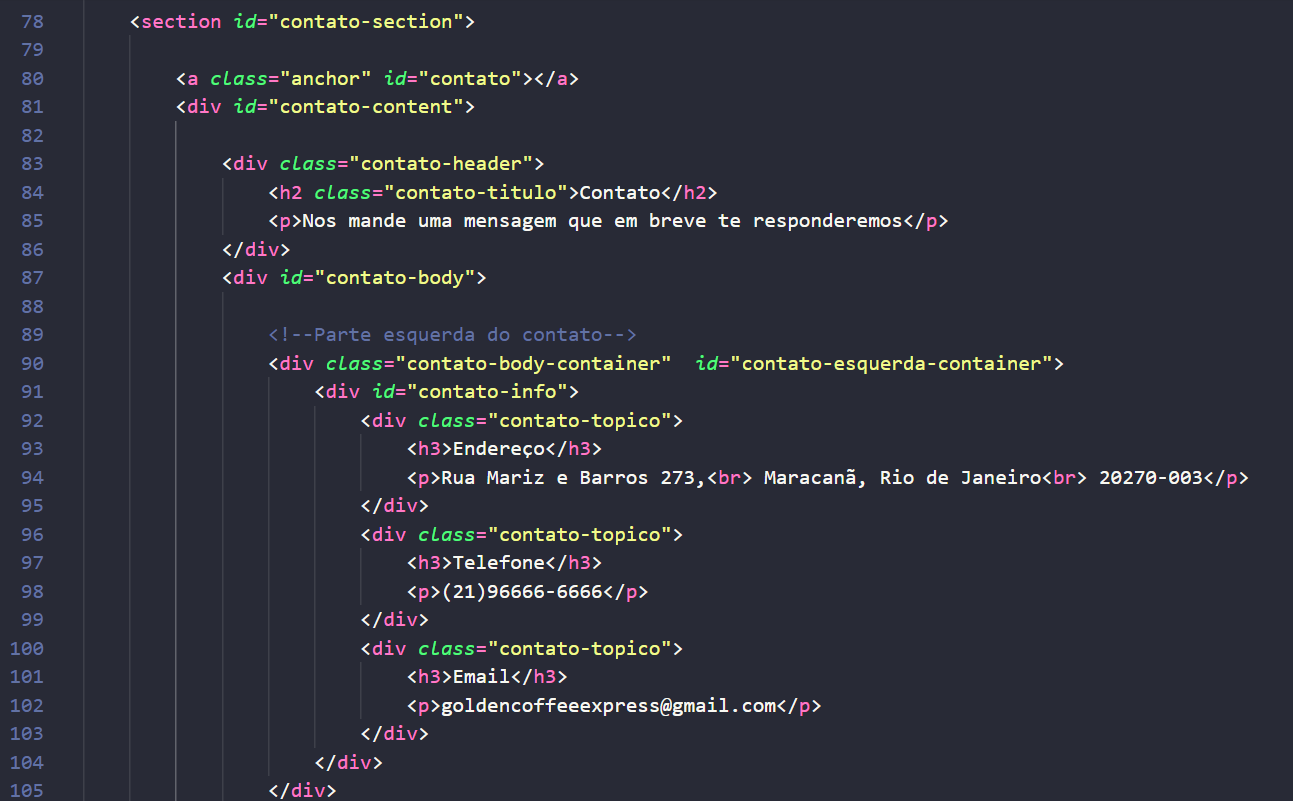
\includegraphics[width=15cm]{Contato HTML 1}
	\caption{Contato HTML 1}
\end{figure}

\begin{figure}[!h]
	\centering
	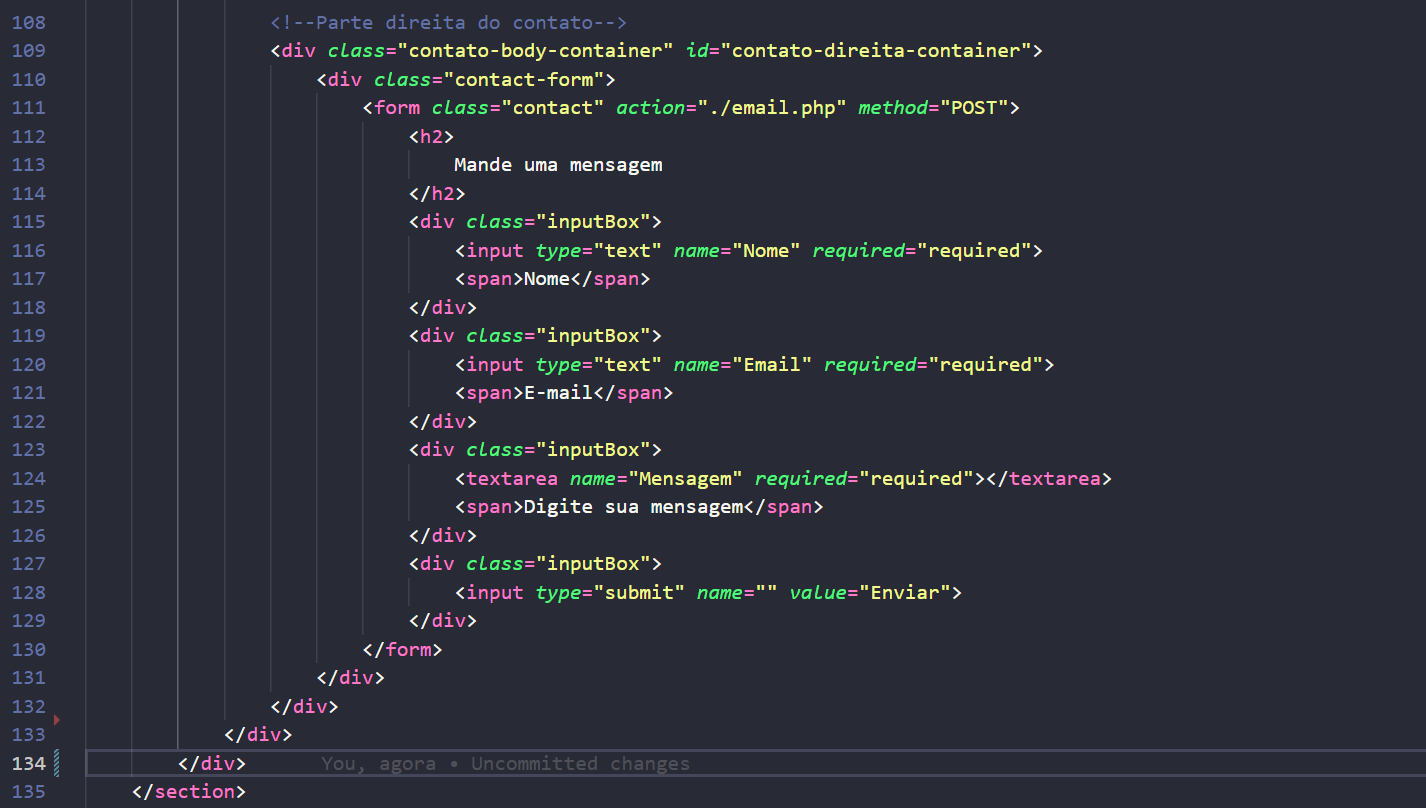
\includegraphics[width=15cm]{Contato HTML 2}
	\caption{Contato HTML 2}
\end{figure}

\begin{figure}[!h]
	\centering
	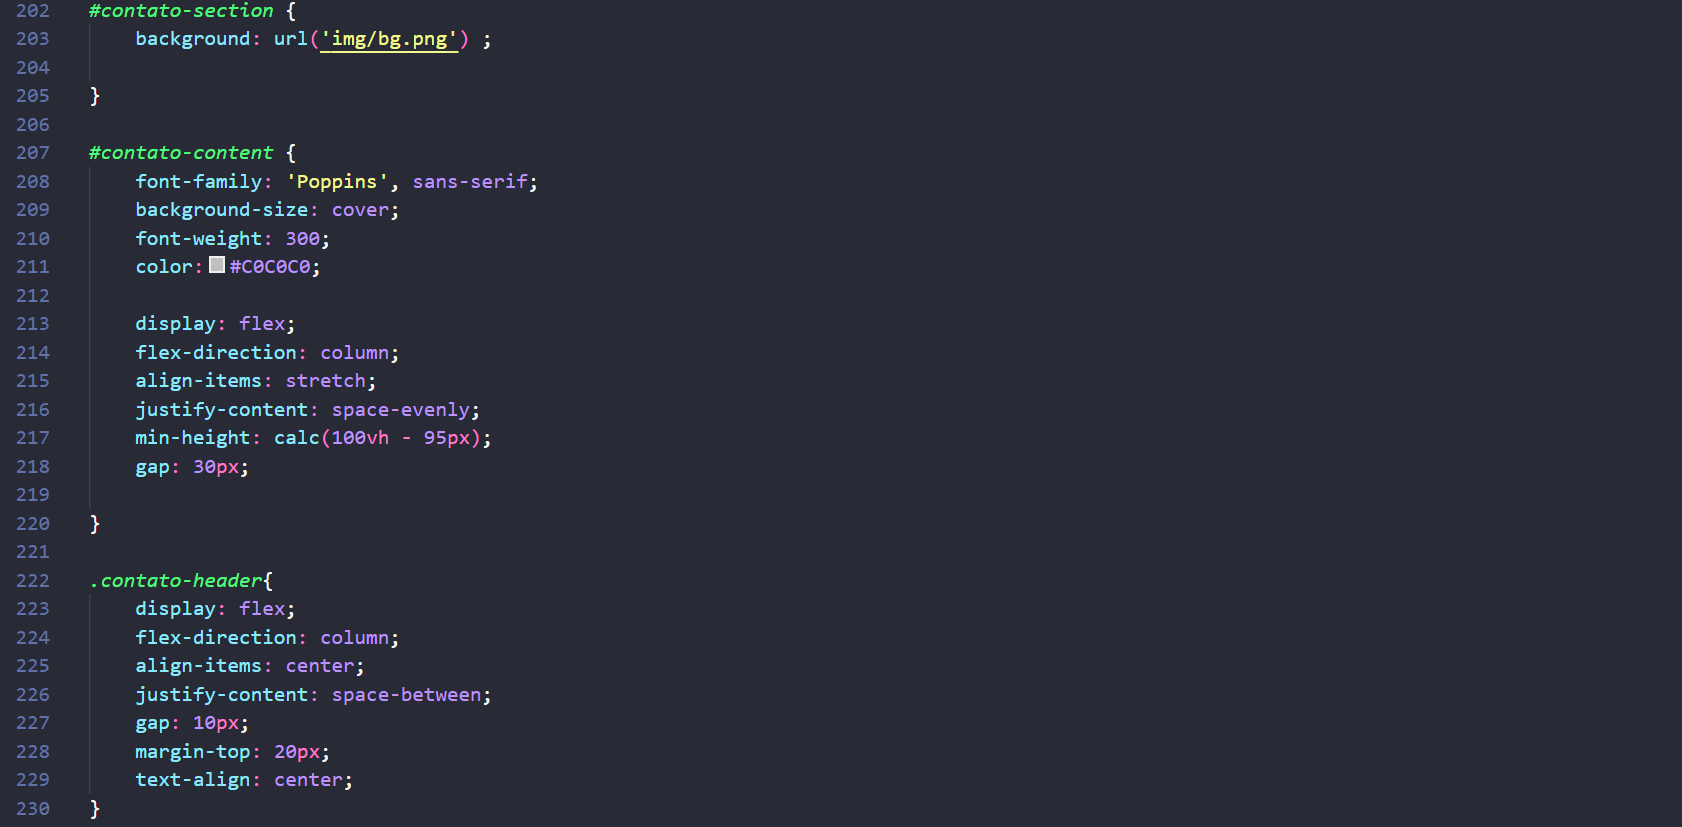
\includegraphics[width=15cm]{Contato CSS 1}
	\caption{Contato CSS 1}
\end{figure}

\begin{figure}[!h]
	\centering
	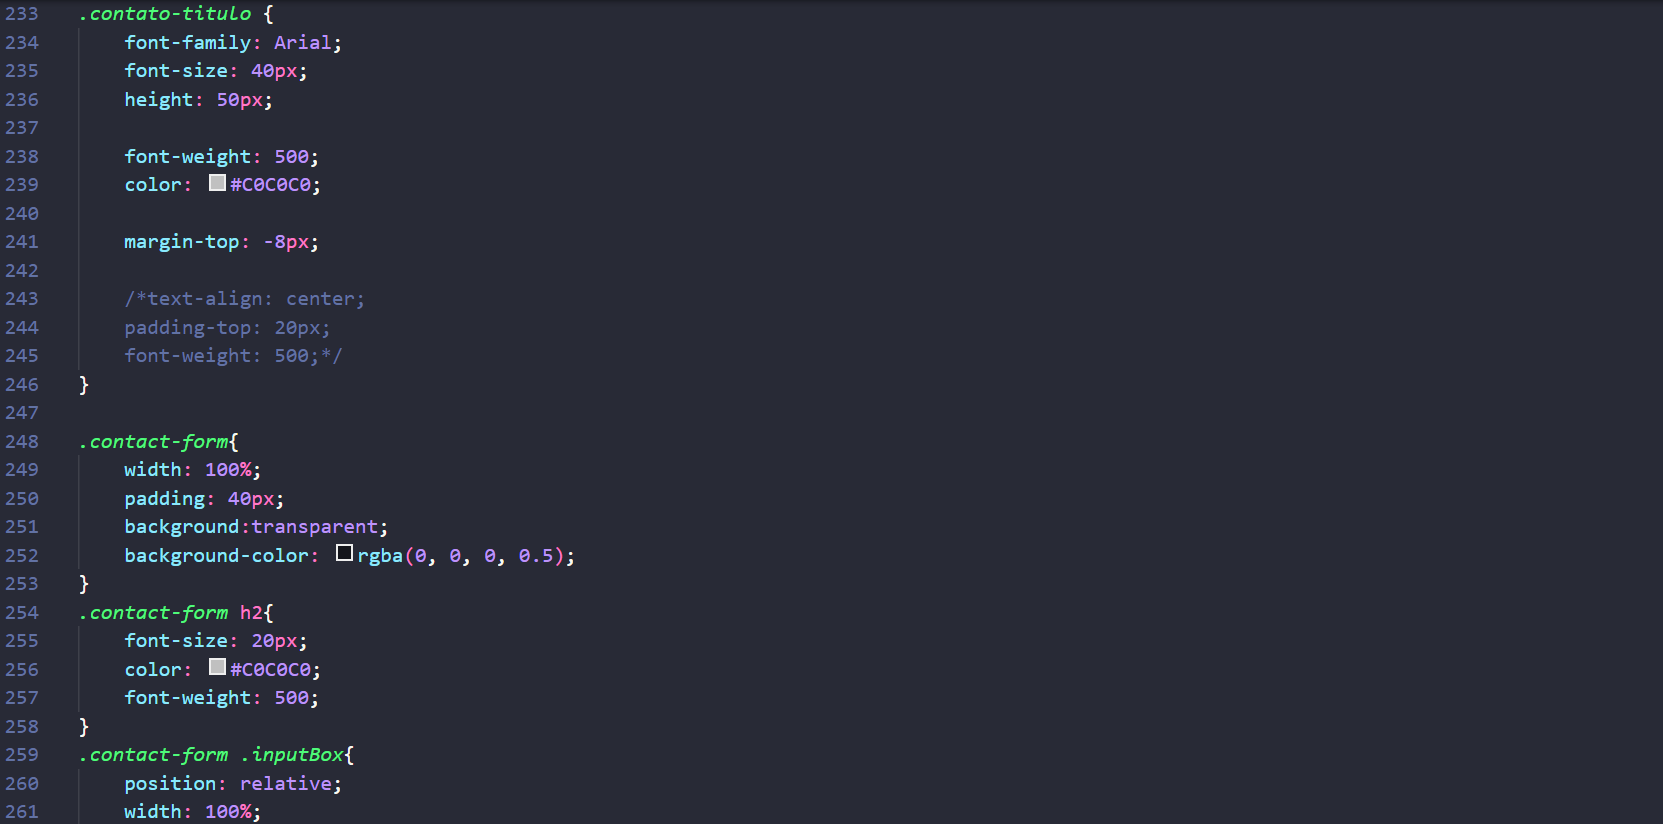
\includegraphics[width=15cm]{Contato CSS 2}
	\caption{Contato CSS 2}
\end{figure}

\begin{figure}[!h]
	\centering
	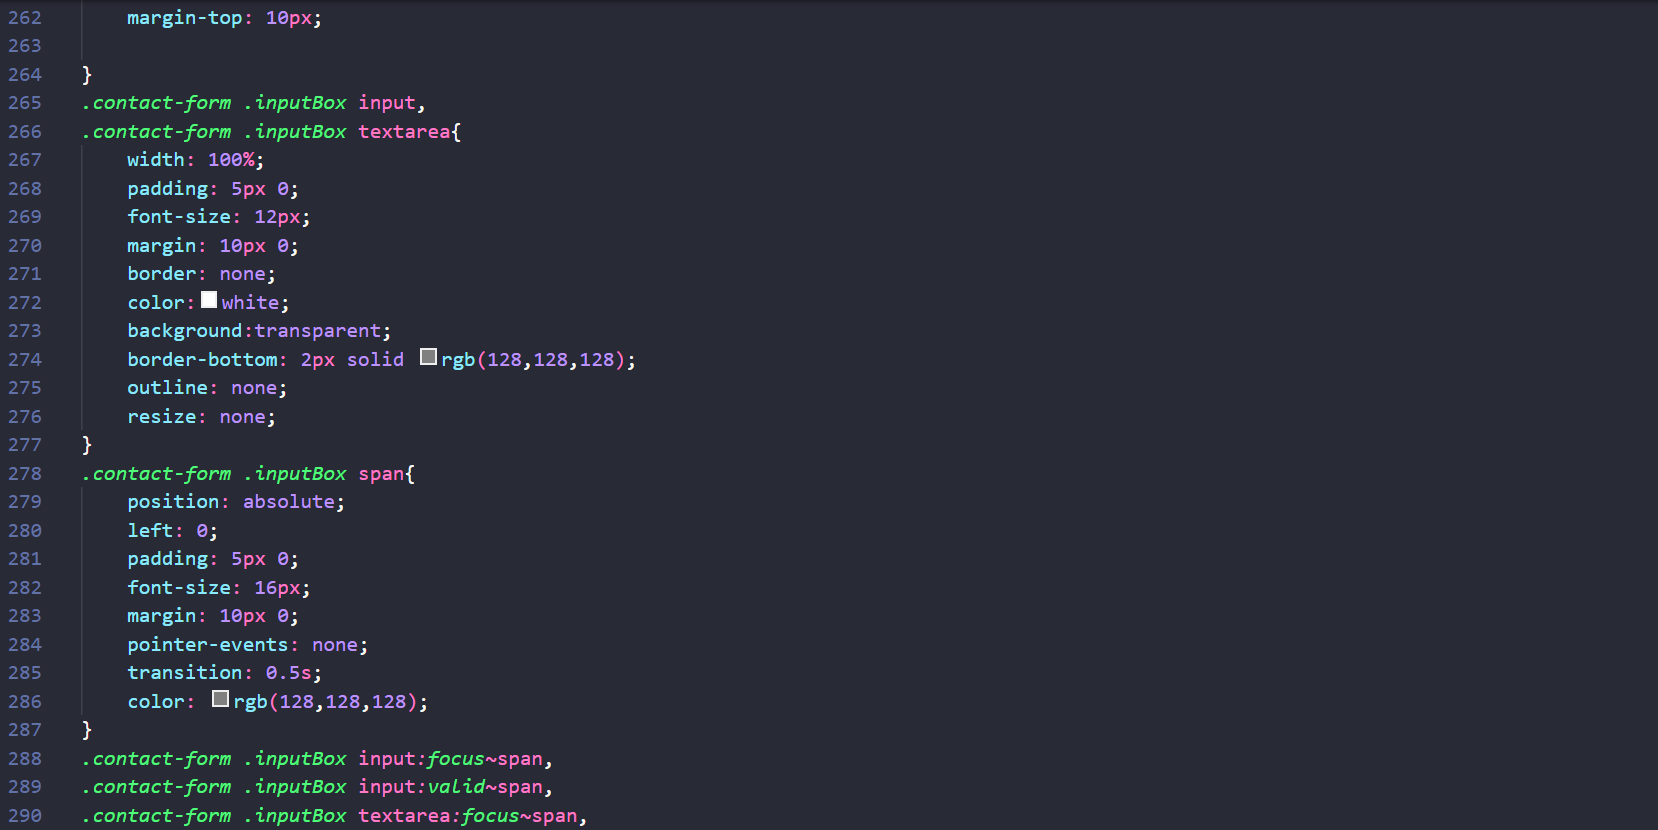
\includegraphics[width=15cm]{Contato CSS 3}
	\caption{Contato CSS 3}
\end{figure}

\begin{figure}[!h]
	\centering
	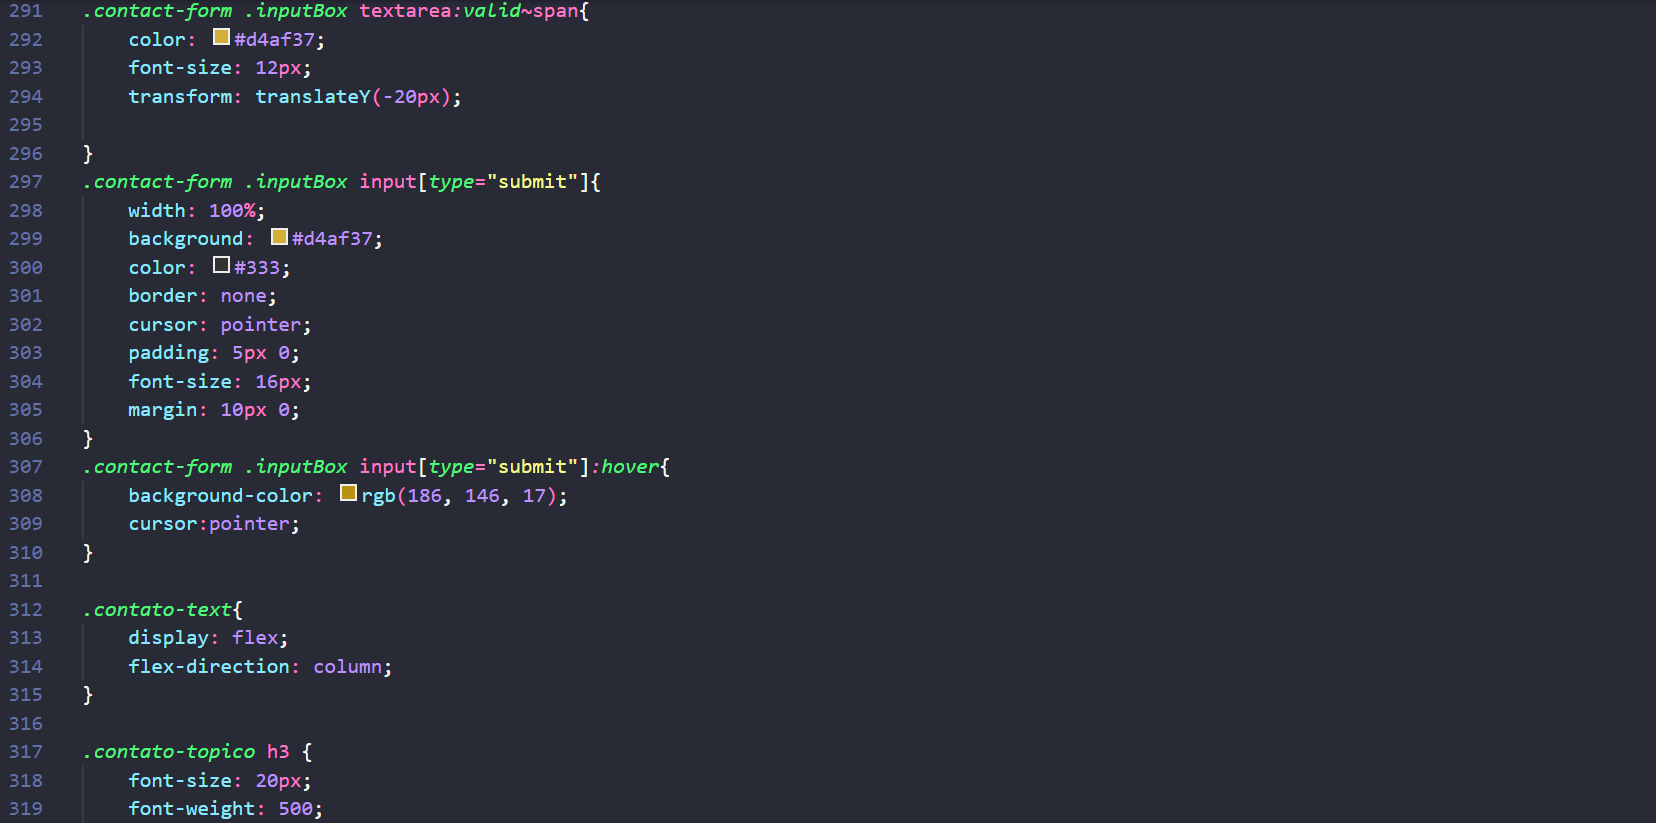
\includegraphics[width=15cm]{Contato CSS 4}
	\caption{Contato CSS 4}
\end{figure}

\begin{figure}[!h]
	\centering
	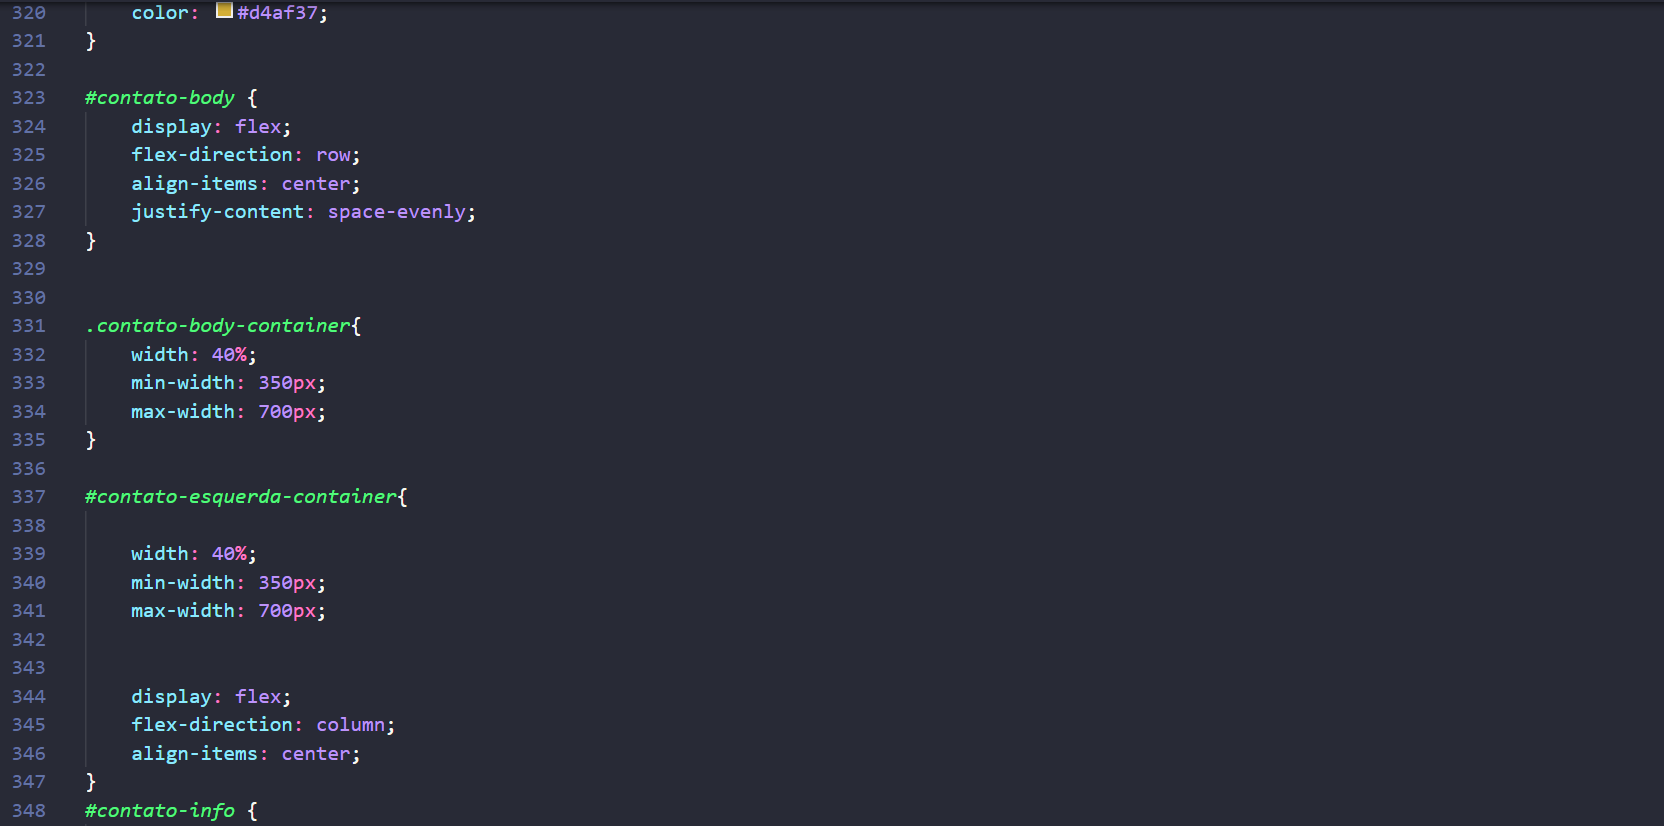
\includegraphics[width=15cm]{Contato CSS 5}
	\caption{Contato CSS 5}
\end{figure}

\begin{figure}[!h]
	\centering
	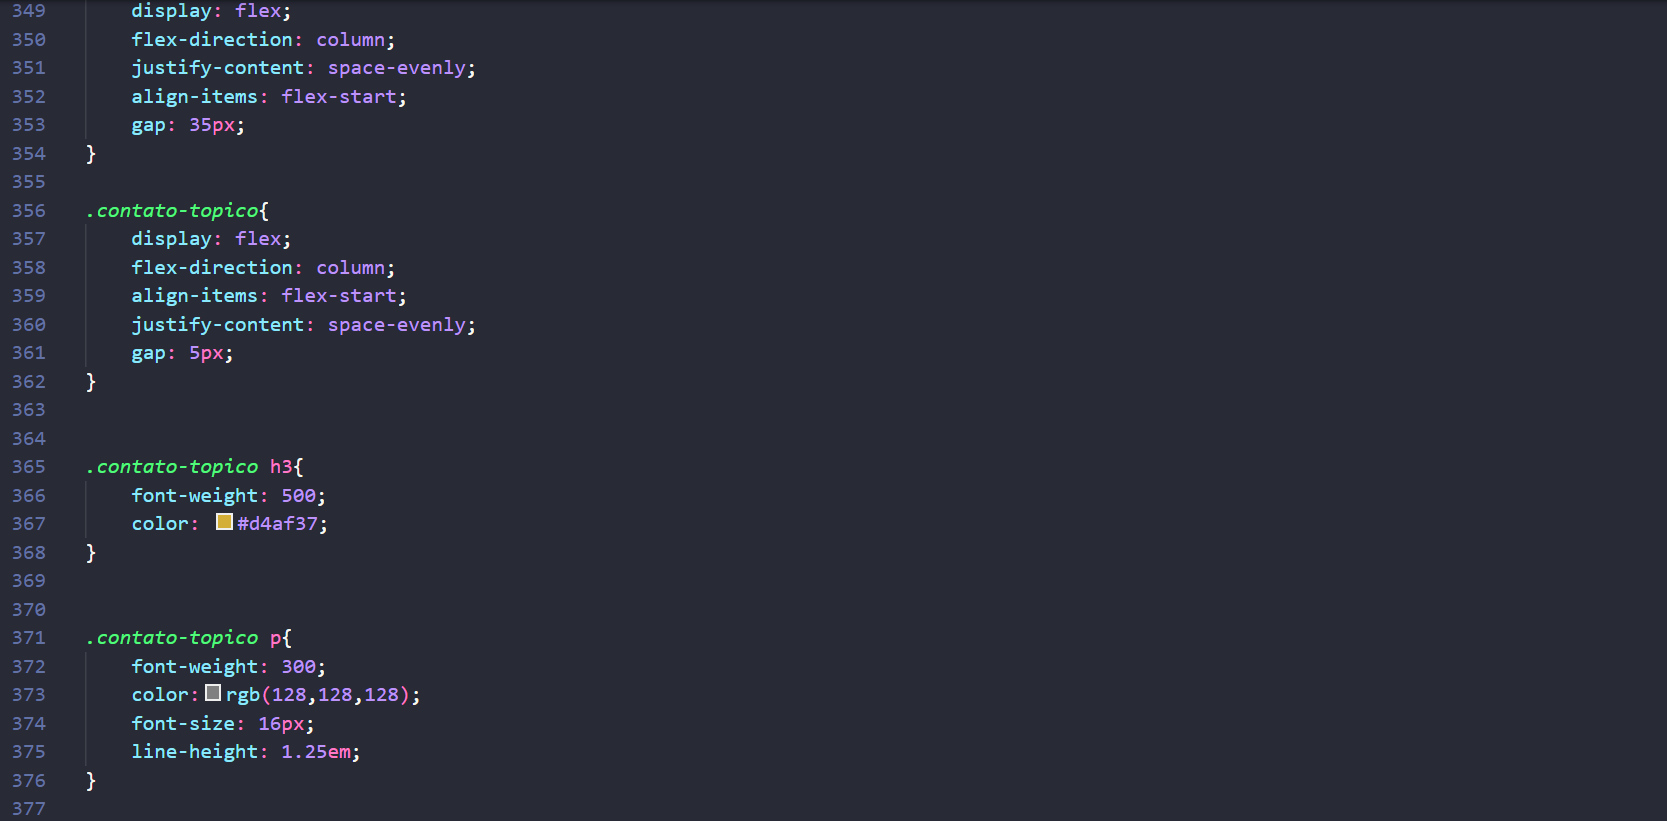
\includegraphics[width=15cm]{Contato CSS 6}
	\caption{Contato CSS 6}
\end{figure}

\begin{figure}[!h]
	\centering
	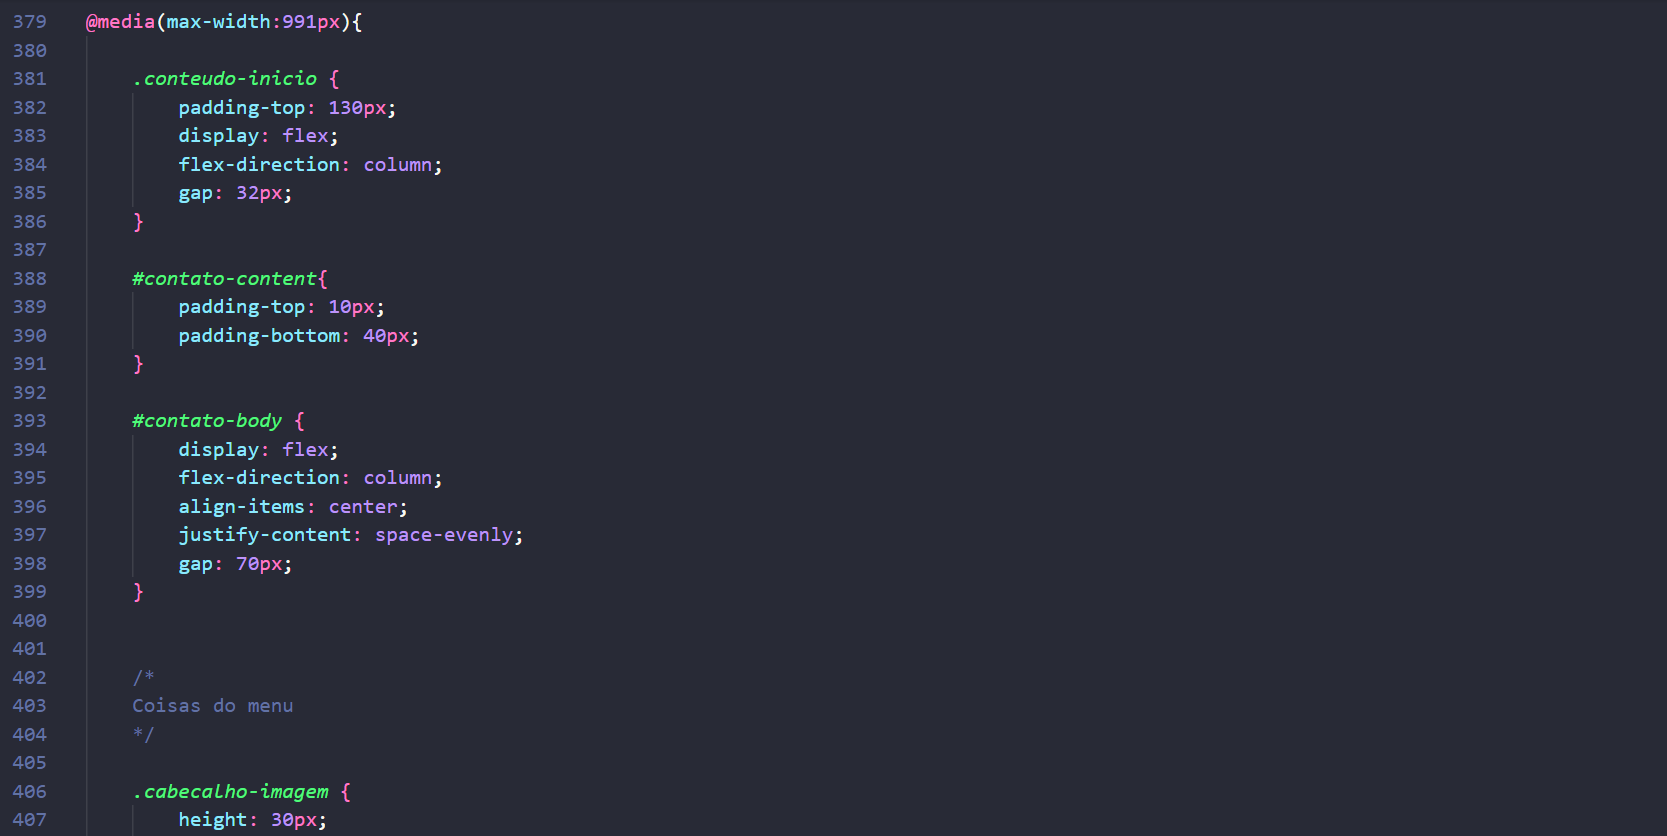
\includegraphics[width=15cm]{Contato CSS 7}
	\caption{Contato CSS 7}
\end{figure}

\begin{figure}[!h]
	\centering
	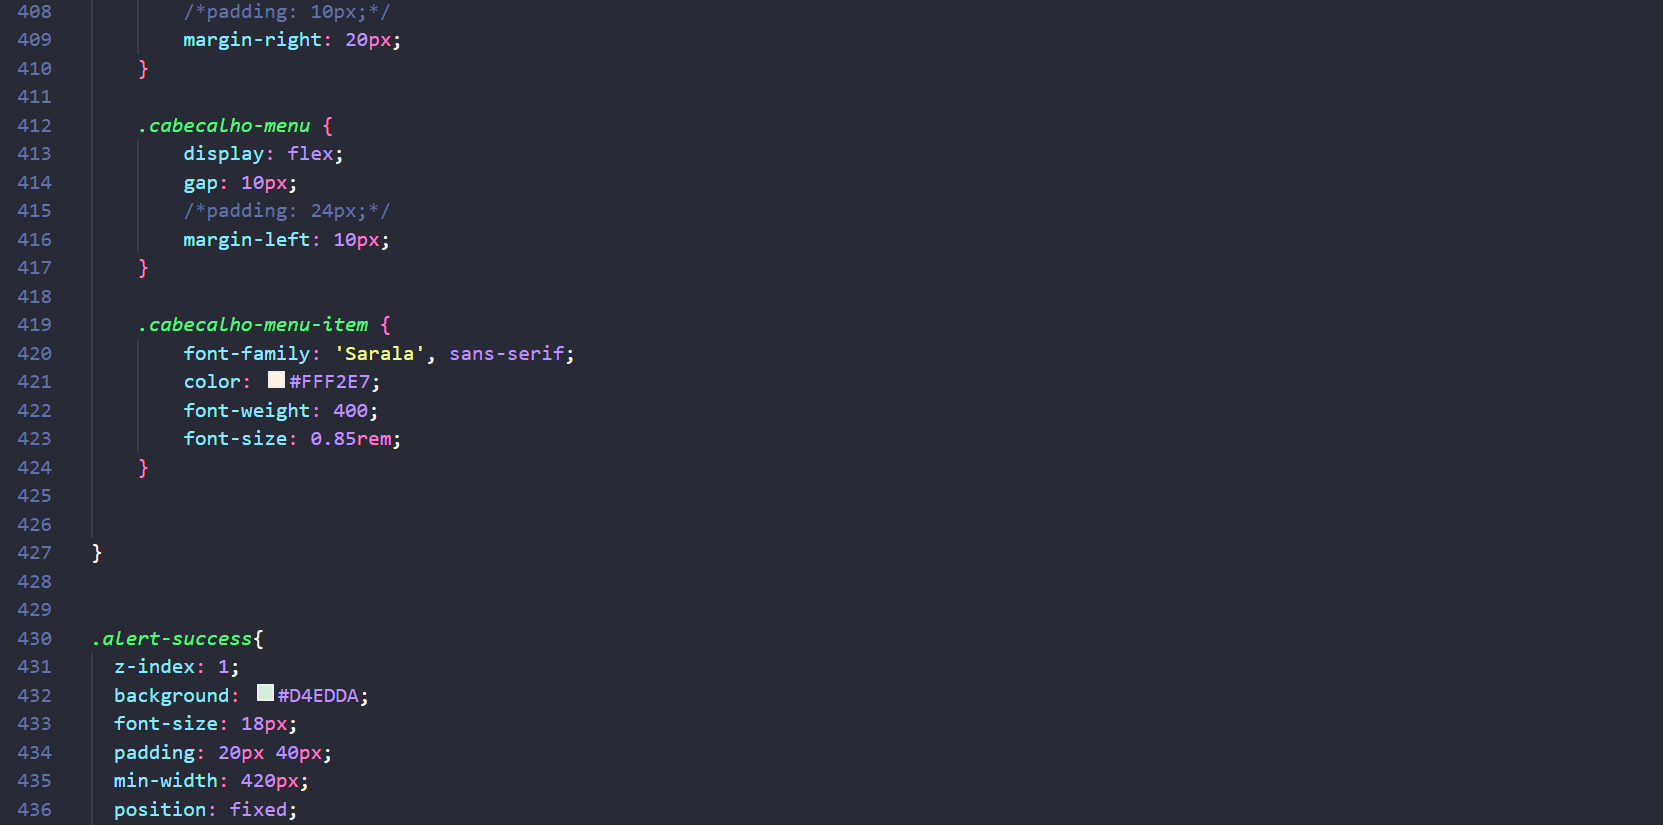
\includegraphics[width=15cm]{Contato CSS 8}
	\caption{Contato CSS 8}
\end{figure}

\begin{figure}[!h]
	\centering
	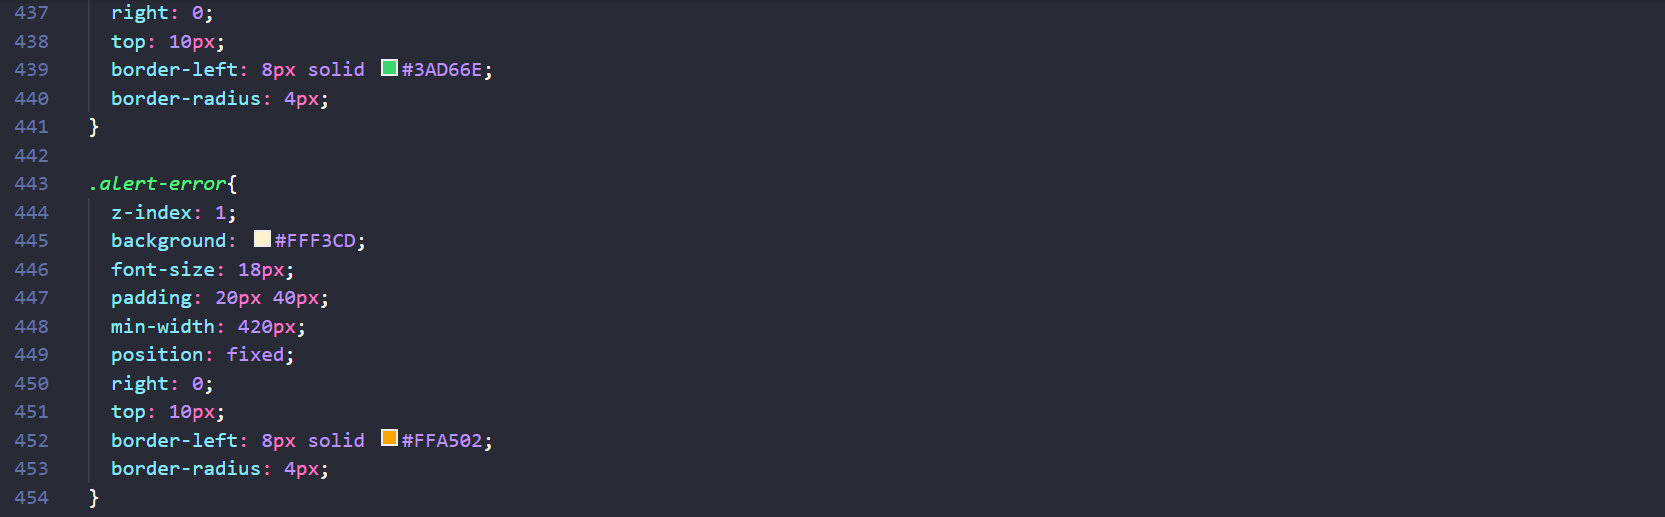
\includegraphics[width=15cm]{Contato CSS 9}
	\caption{Contato CSS 9}
\end{figure}

\begin{figure}[!h]
	\centering
	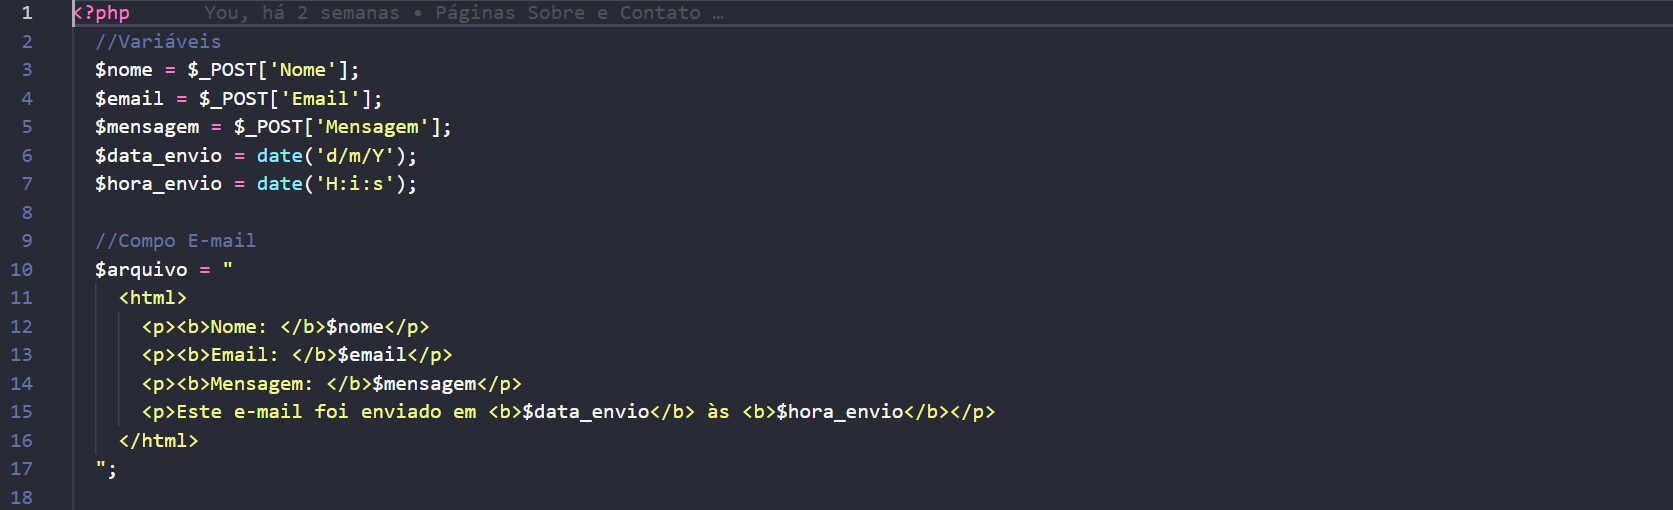
\includegraphics[width=15cm]{Contato PHP 1}
	\caption{Contato PHP 1}
\end{figure}

\begin{figure}[!h]
	\centering
	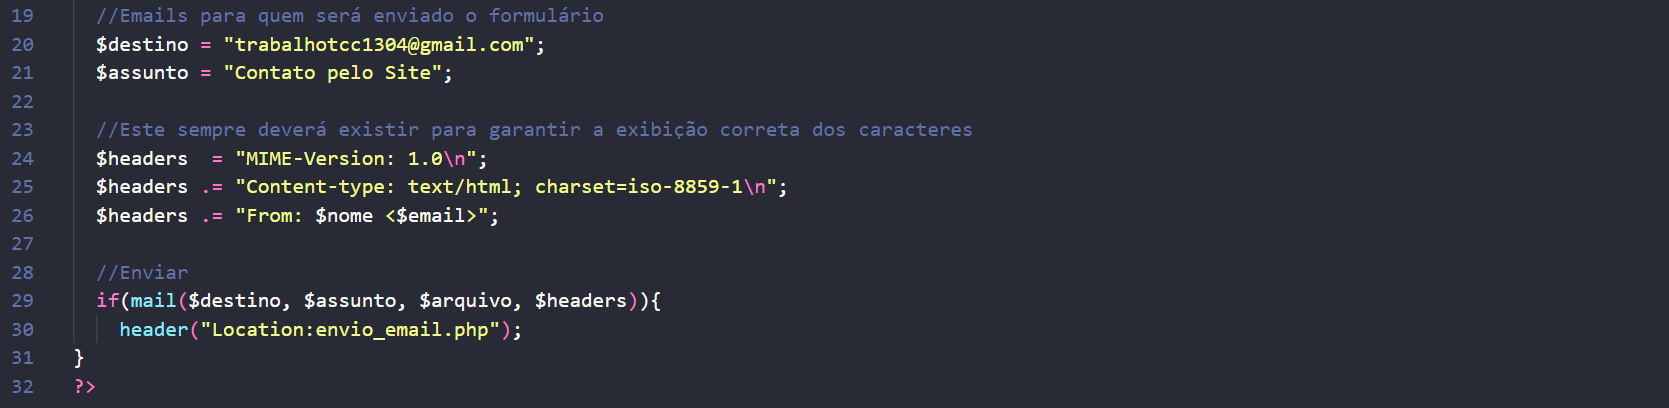
\includegraphics[width=15cm]{Contato PHP 2}
	\caption{Contato PHP 2}
\end{figure}

\section{Funcionalidade de Login}